\chapter{Generation of Seed Light}\label{generationOfSeedLight}

In this chapter, I will discuss the design and construction of the master laser. I built the master laser system beginning in 2010. Initial work on the master laser was completed by Chris Erickson before I joined the project. He ordered many of the components and did some of the early work to begin to assemble the laser.

The main goal of the master laser system is to produce a stable oscillator from which the signals used to injection lock the slave lasers can be derived. It must have a reasonably narrow linewidth (narrow enough to resolve and it must operate with a single spatial mode. The master laser must also be tunable over a large enough range that it can be   

The main concern regarding the master laser is that we need to get it to the right wavelength. Most of the processes in this chapter involve some means of maximizing the likelihood that we can get the master laser to oscillate at a frequency at which we can run the experiment. The basic means of controlling the master laser are
\begin{itemize}
\item Diode selection
\item Temperature 
\item Current
\item Coarse adjustment of grating using threaded actuators
\item Electronic adjustment of grating using piezoelectric actuators
\end{itemize}
Each of these factors is interdependent and, in general, the adjustment of one usually involves adjusting all the others. However, as we will see, many of the steps I did to build the master laser had the end goal of making sure that we could get the laser to the right wavelength with ever greater control and accuracy. 

\section{Stabilization of Master Laser}
\subsection{Master Laser Layout}
The master laser is a 408 nm extended cavity diode laser (ECDL). It consists of a laser diode mounted in a temperature-controlled housing from the Thorlabs LDM21 family of products. It is collimated by a small, aspherical lens (Thorlabs C570TM-A). The master laser ECDL also has a grating mounted outside of the temperature-controlled housing. The grating is mounted on a Thorlabs KC1-PZ piezoelectric kinematic mount, which is attached to the laser via a series of rods. A picture of the master laser can be seen in Fig.\,\ref{master_laser_photo}, while a picture of the inside of the housing can be seen in Fig.\,\ref{master_laser_interior_photo}.

\begin{figure}
\centerline{
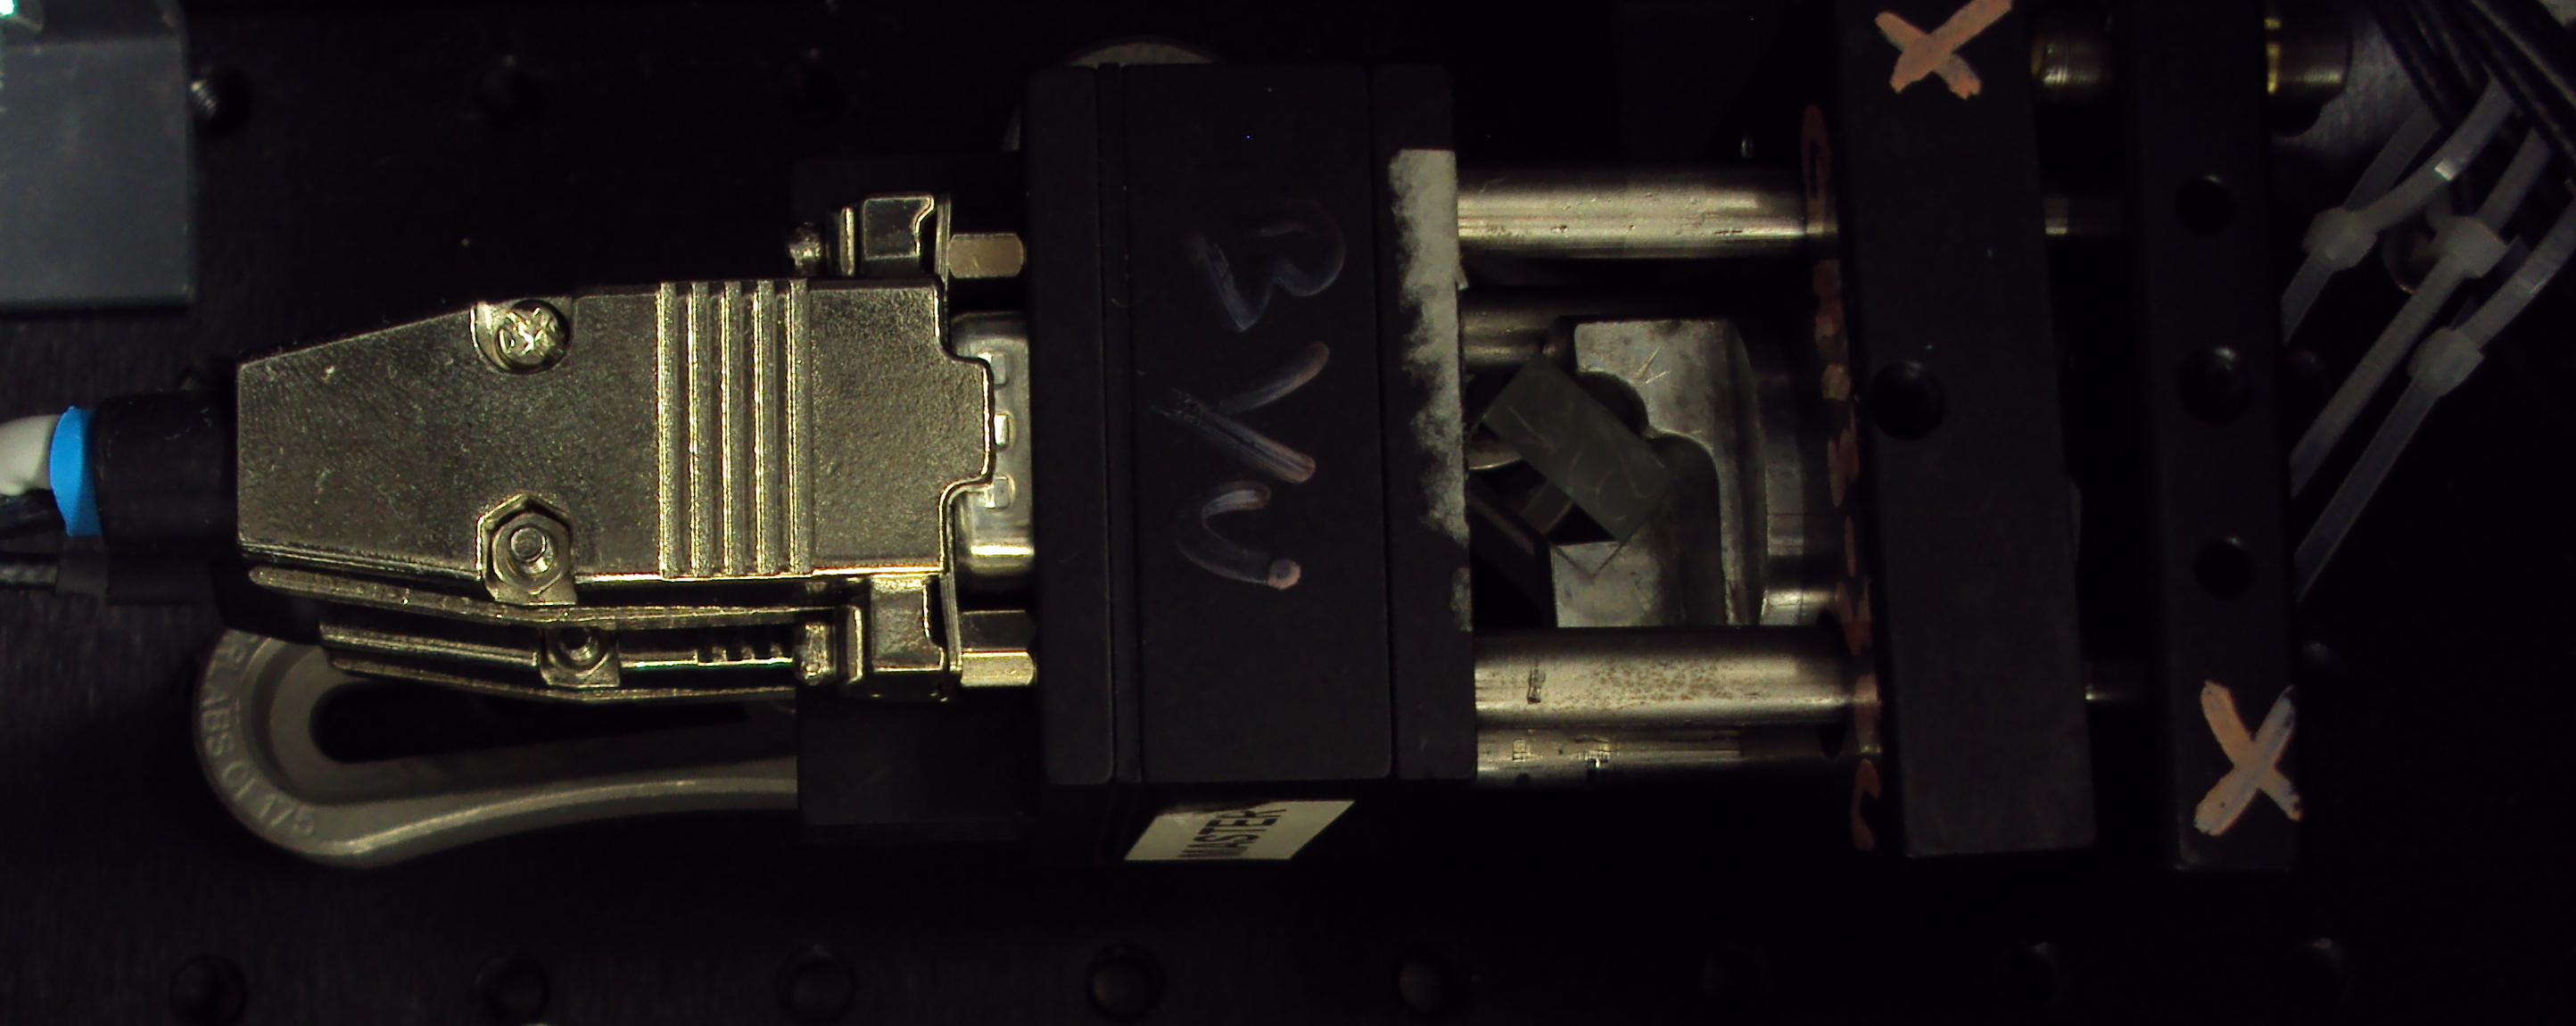
\includegraphics[width=0.95\textwidth]{master_laser.JPG}}
\caption[Photograph of Master Laser]{\label{master_laser_photo} The master laser system. The diffraction grating that provides feedback to the laser is mounted on a custom machined grating holder that is attached to the Thorlabs KC1-PZ piezoelectric kinematic mount. . I initially tried several other configurations. However, after several iterations, I found that the use of the metal rods to provide direct  mechanical coupling between the laser and grating mount were necessary for stable, single-mode operation. I also found through trial and error that placing the grating a distance of $\sim$4 cm from the aperture seemed to work for this particular laser.}
\end{figure}

\begin{figure}
\centering
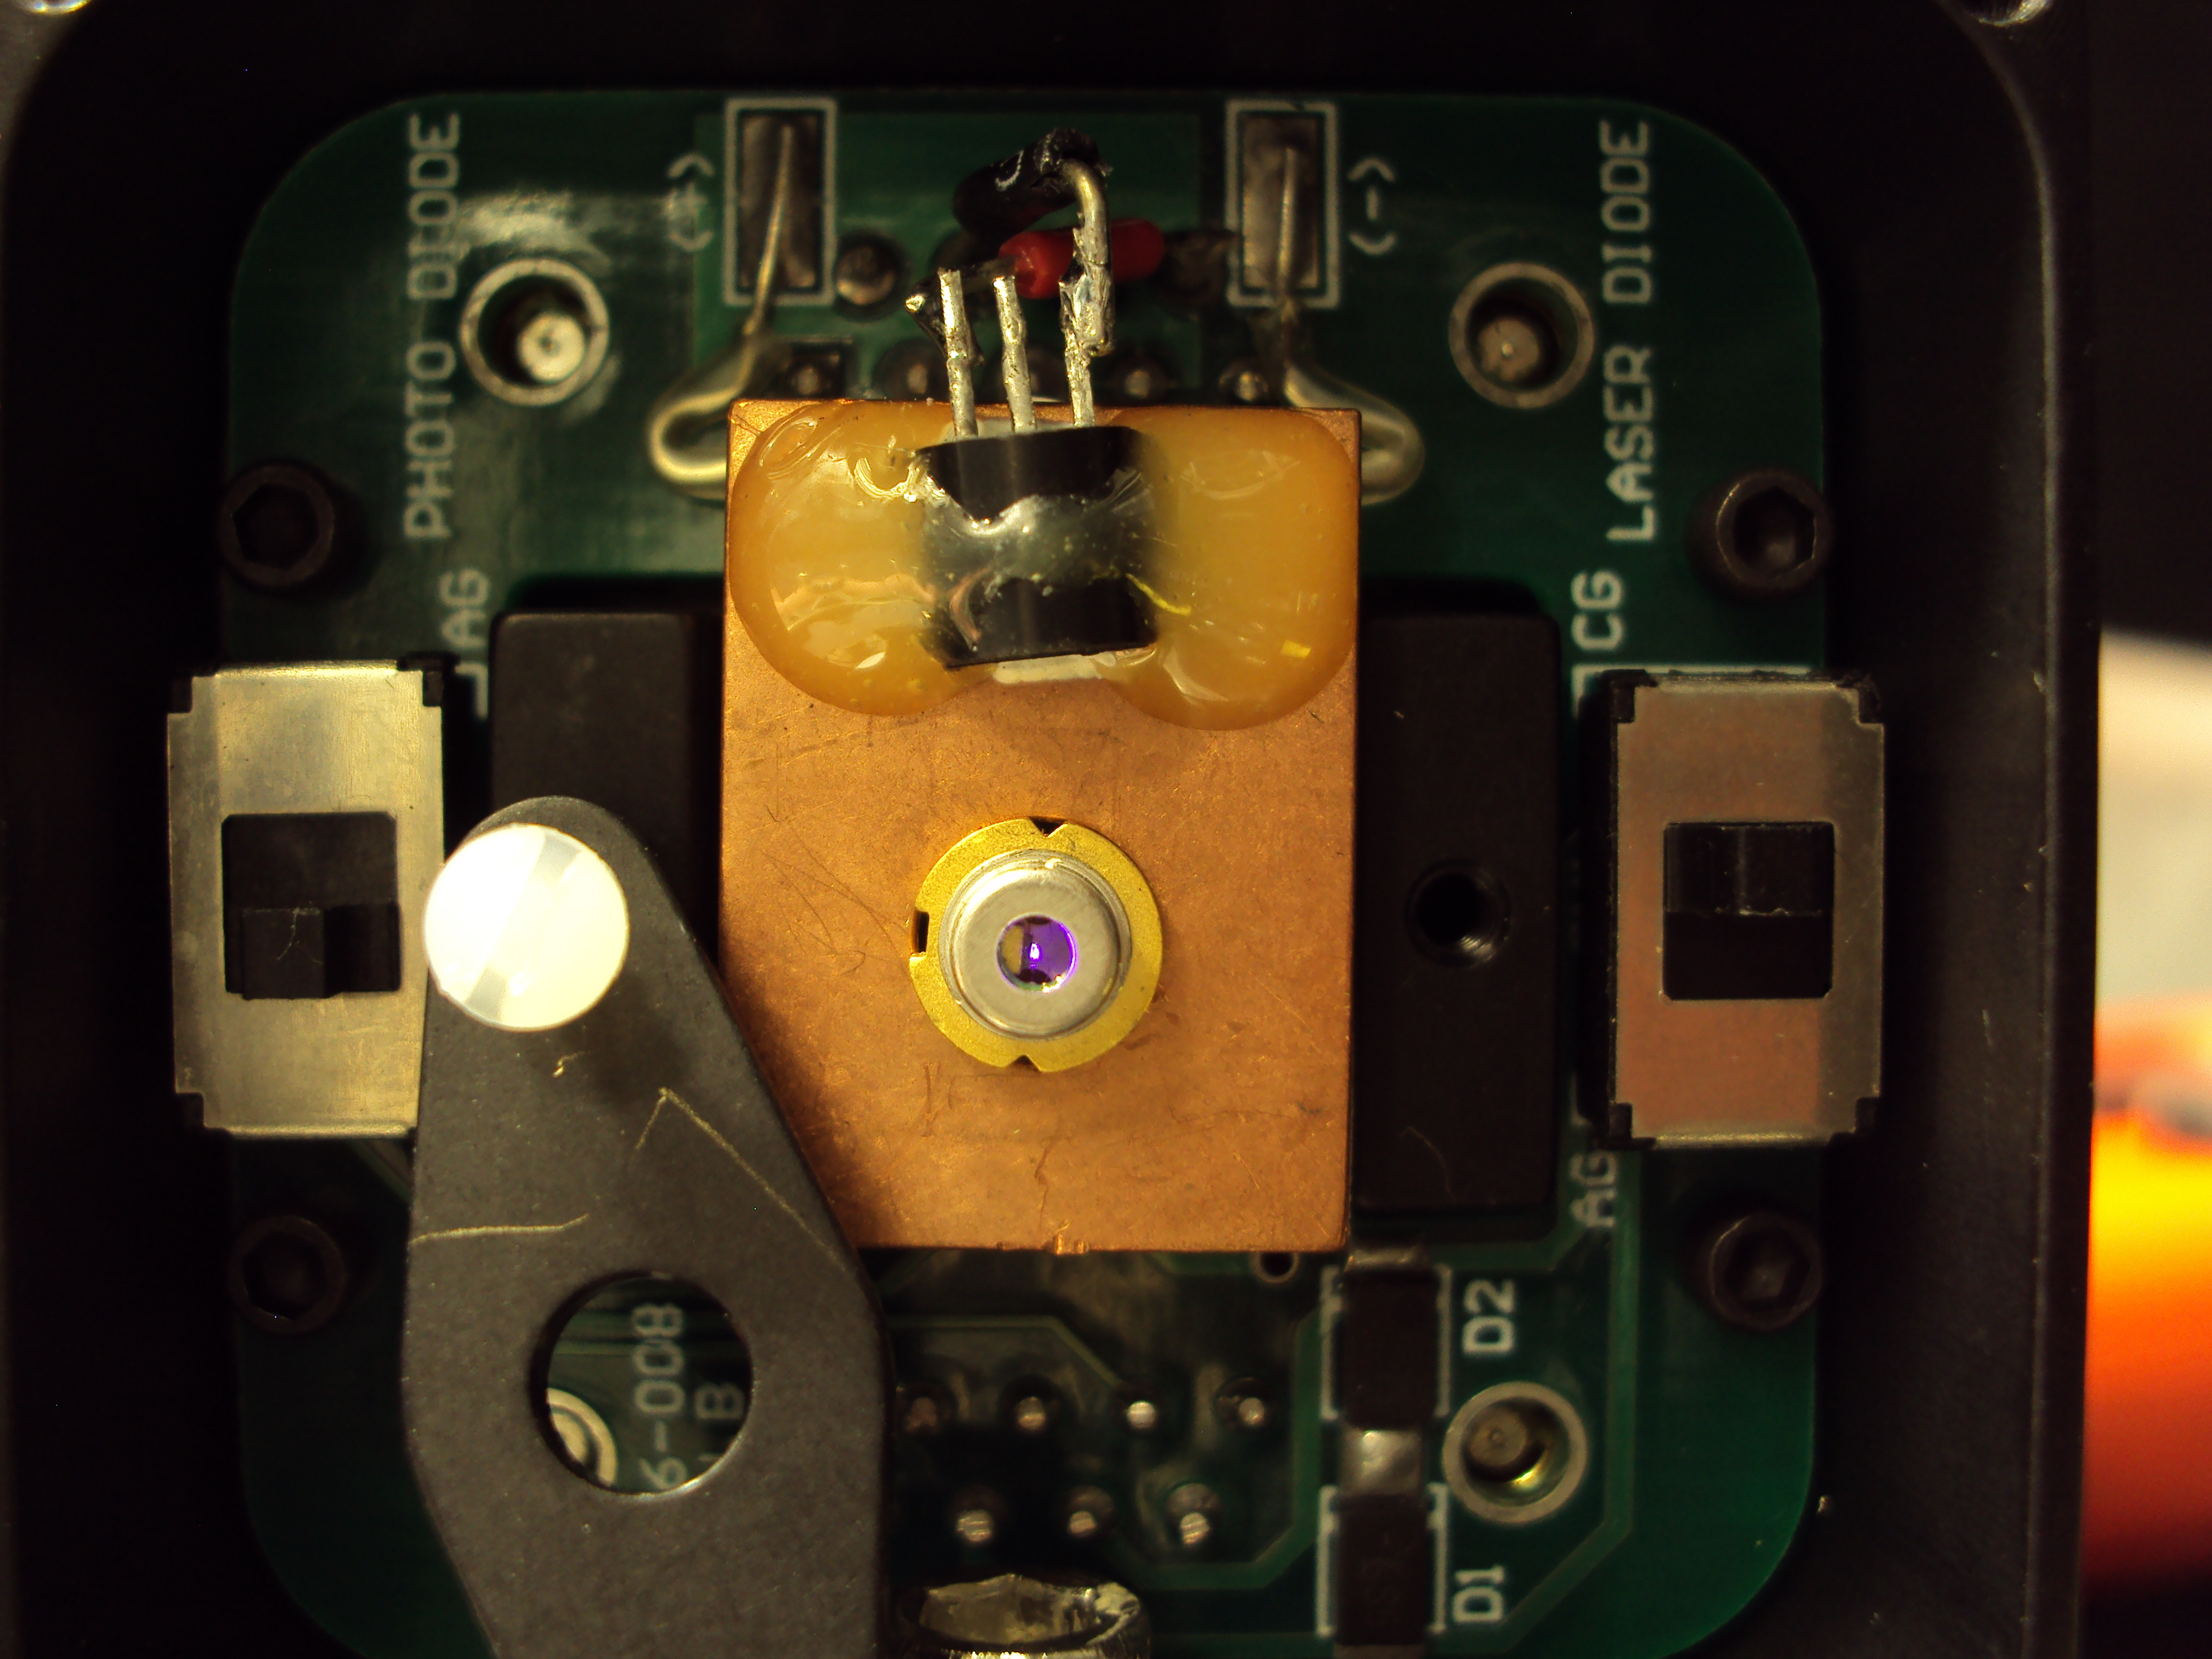
\includegraphics[width=1\textwidth]{laser_on_in_housing.JPG}
\caption[Photographs of Master Laser Components]{The master laser in its housing and the diffraction grating before it was installed (inset). We modified the housing to include an additional temperature sensor (the AD592), which can be seen glued to the top of the copper plate.}
\end{figure}
%why did we do the rods? Do I have it in my notes?
%do I mention how we ran them sideways? I mean, we had holes in the sides and all that? 

\subsection{Master Laser Diode Selection}
\label{masterLaserDiodes}
The diode used in the master laser is a single-spatial mode InGaN diode. Its model number is Mitsubishi ML320G2. The master laser was wavelength-selected by the distributor (i.e. the distributor performed measurements and binned the parts based on their output wavelengths; we then ordered lasers from their 408 nm bin). The diode is very similar to the diode lasers used in Blu-ray players. 
In fact, we also bought 30 diodes on eBay that had been removed from actual Blu-ray or HD-DVD players as backup diodes. We measured the free running wavelengths of these diodes in order to bin them ourselves using techniques that I will describe in Section\,\ref{gratingSpectrometerWavelengthMeasurements}. Some of these diodes were ultimately used in the slave lasers, whose configuration will be described in Section\,\ref{initialSlaveConfiguration}.


%Mark? Did he do this? 

The selection of laser diodes required a few iterations before I found diodes that would work properly. I initially tried to build the master laser using a non-wavelength-selected Sharp GH04020A2GE low power diode, which I could not stabilize for unknown reasons. I quickly switched to a non-wavelength-selected Sharp GH04P21A2GE diode for the master laser. However, this laser's free-running wavelength at 25$^\circ$C was far too low. In order to tune this diode to the correct wavelength, I found that I had to maintain the diode at a temperature of $\sim$60$^\circ$C. Running at such a high temperature resulted in degradation of the diode and loss of power over the course of a few months. It was this experience that prompted me to use wavelength selected diodes. In this way, I was able to get a laser that could lase at the wavelength we needed without having to risk seriously diminishing the operational lifetime of the laser.

\subsection{Grating Spectrometer Wavelength Measurements}
\label{gratingSpectrometerWavelengthMeasurements}
In order to tune the master laser to precisely the correct wavelength and to measure the room temperature free running wavelength of the uncharacterized lasers (i.e. the lasers that were bought on eBay and later used in the slave lasers), I used a compact grating spectrometer from the Ocean Optics USB2000 series to measure the center frequency of the free-running laser diodes. This spectrometer uses a diffraction grating to separate light based on its constituent wavelenghts. Light scattered off the diffraction grating is detected by a CCD array consisting of 2048 pixels that is also enclosed in the spectrometer. The average difference in wavelength between adjacent pixels is $\sim$.061 nm. % This according to /research/octave/ooSpectrumData12Sep/MasterFile.m using the lambdas variable defined in there.

I tried several techniques to maximize the resolution and accuracy of these measurements. The center wavelength of the bare diodes changed only a few nanometers over the entire range of possible temperatures and currents. In order to ensure accurate absolute wavelength measurements, we calibrated to a mercury source both before and after looking at the spectra of the various lasers. We feel confident in our calibrations since mercury conveniently has spectral lines at 405 and 436 nm, which are close to our target wavelength of 407.771 nm. A typical before and after calibration spectrum taken using the mercury lamp can be seen in Figure\,\ref{calibrationData}. When analyzing the peaks produced by the laser on the grating spectrometer, we fit the measured data to a Gaussian distribution in hopes of squeezing out some sub-pixel level resolution of the peak location. Examples of this type of analysis are shown in Figures\,\ref{Temperaturespectra} and \ref{wavelengthselected}.

%diagram of which method to use where? 
%The basic 

%\subsection{Master Laser Temperature and Current Selection}

The temperature and the current of the laser are two of the main means we have for affecting the wavelength of the master laser. Using a grating spectrometer, we measured the center wavelength of the bare laser (i.e. no grating feedback or extended cavity).


We have data on the wavelength dependence on temperature and current for our laser. This data is plotted in Fig.\,\ref{3dCurrentandTgraph}. We see that the variation of the center wavelength of the laser is roughly linear over reasonable values of temperature and current.

\begin{figure}
\centering
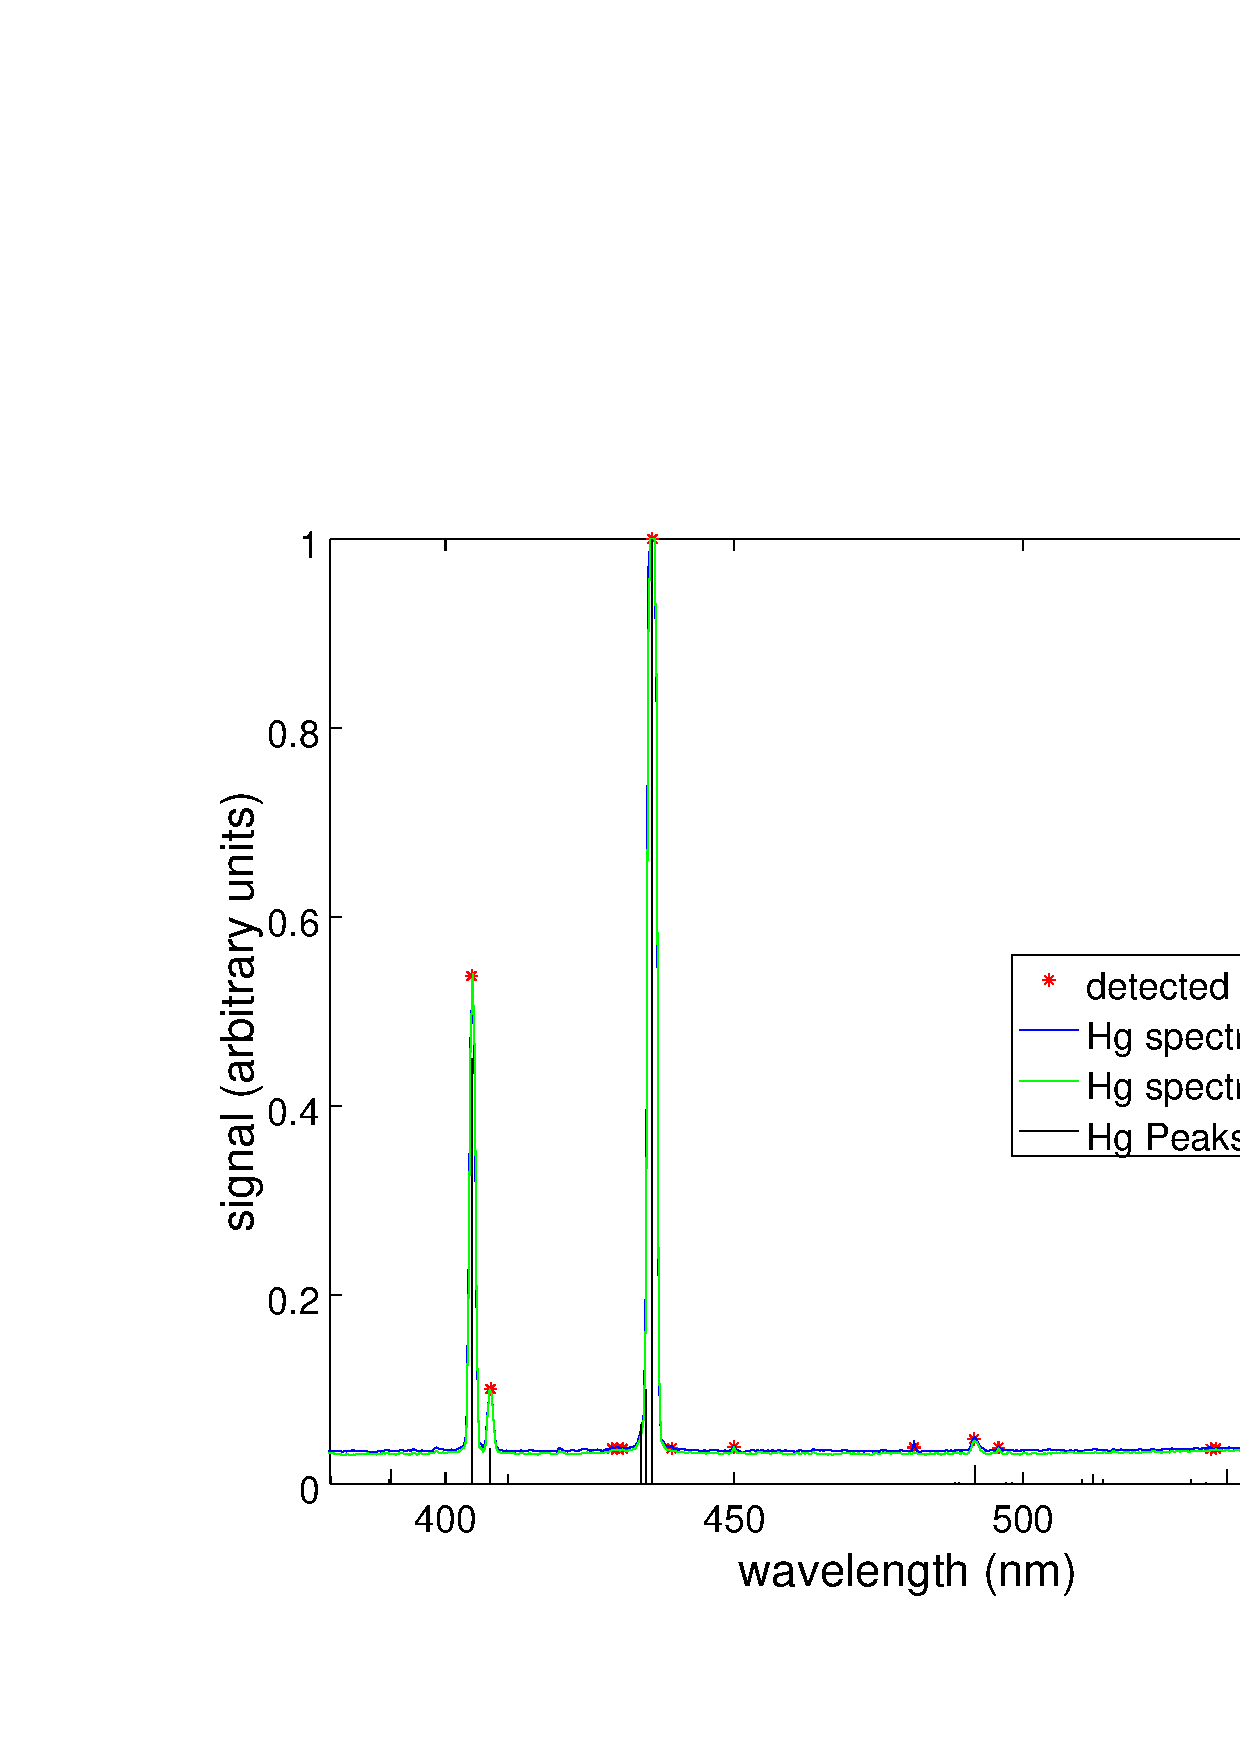
\includegraphics[width=0.95\textwidth]{calibrationData} 
\caption[Calibration spectrum from Hg Lamp]{\label{calibrationData} Data from the calibration using the mercury lamp. I deliberately allowed some of the farther away peaks to saturate in order to improve our signal for the peaks near 408 nm. The black lines represent spectral lines taken from the NIST Atomic Spectra Database\cite{NISTasd}. The average of the premeasured and postmeasured Hg spectra was sent through an Octave script I wrote that automatically identified peaks in the spectrum, displayed the peaks, and then allowed the user to select which peak in the NIST Hg spectrum these peaks corresponded to. The peaks found by this script are displayed with the label, ``detected peaks in measured spectrum.''}
\end{figure}

\begin{figure}
\centering
\begin{subfigure}[b]{0.55\textwidth}
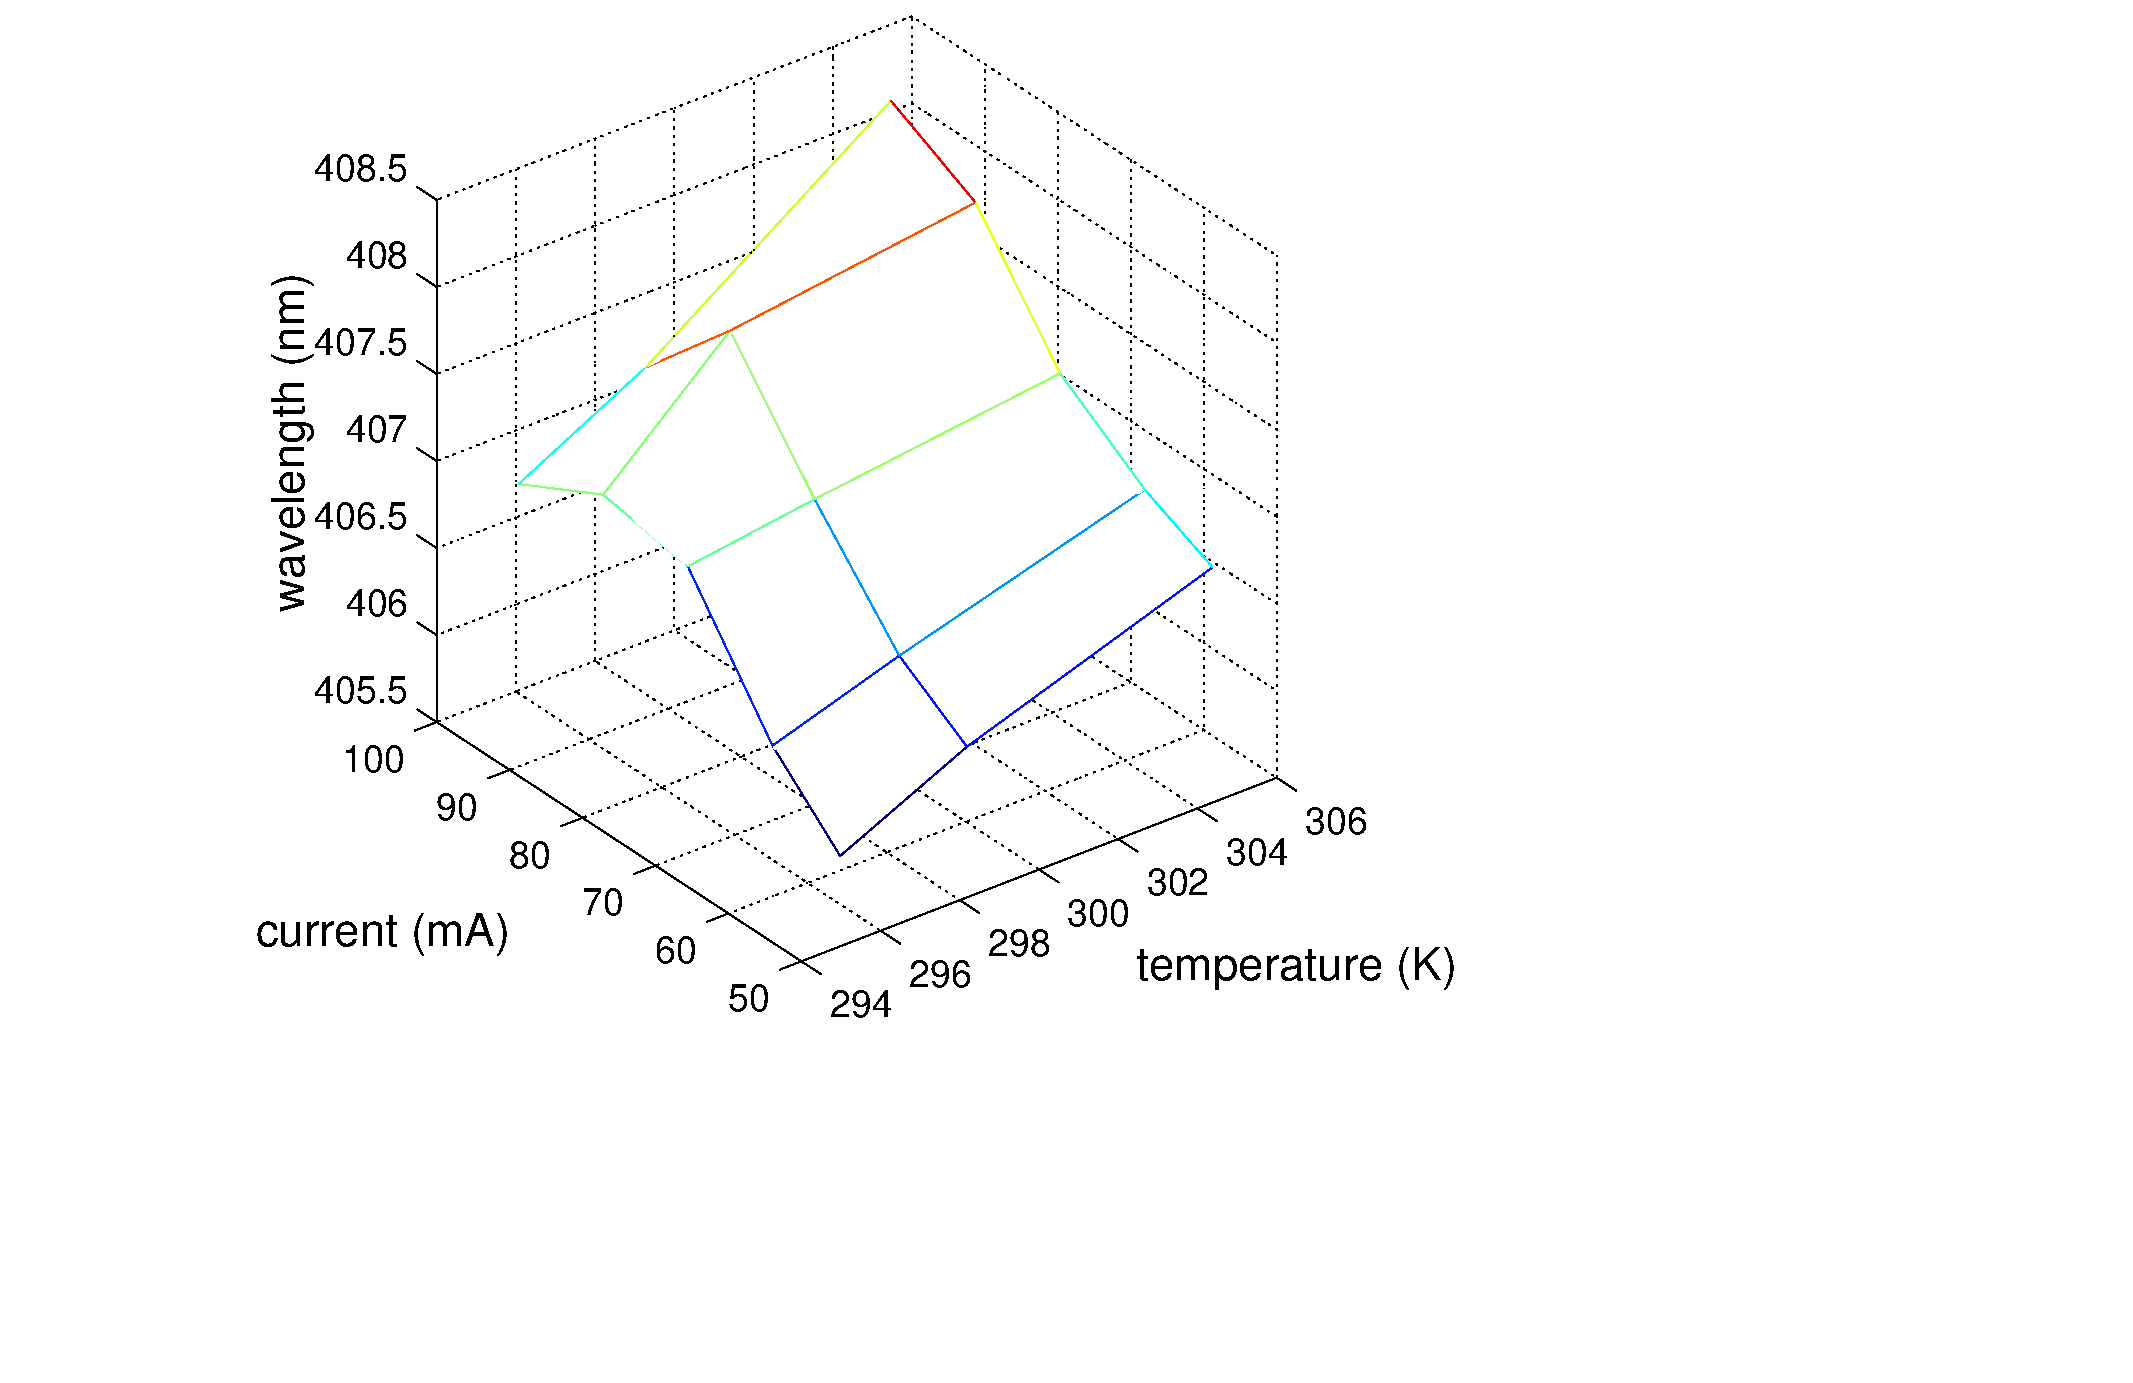
\includegraphics[width=1\textwidth]{TVlambda3} 
\label{currentandT:sfiga}
\end{subfigure}
\begin{subfigure}[b]{0.40\textwidth}
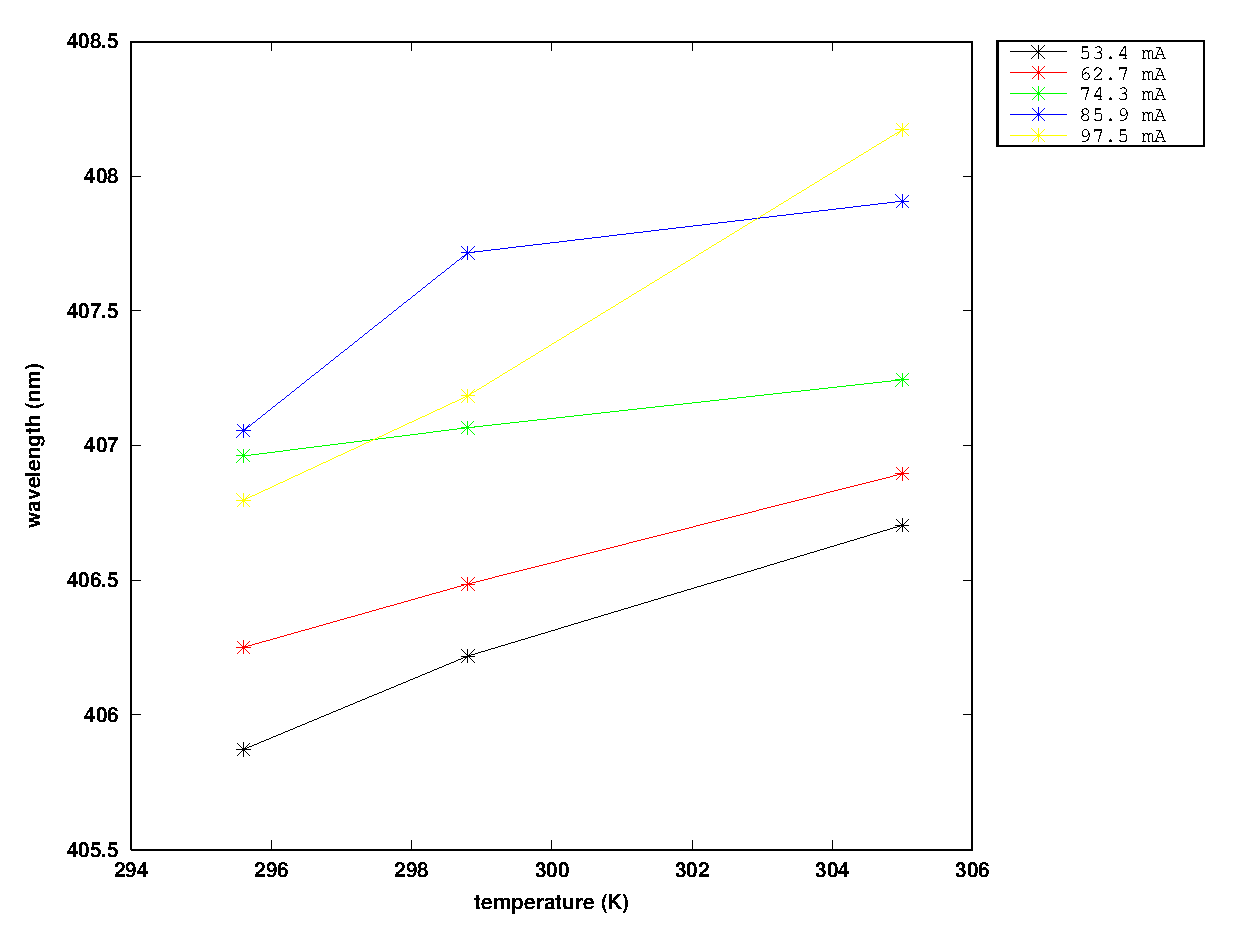
\includegraphics[width=1\textwidth]{TVlambda2}
\label{currentandT:sfigb}
\end{subfigure}
\caption[Graph of Temperatures and Currents]{\label{3dCurrentandTgraph} Representative data of the free-running wavelength of our master laser as a function of nominal current and nominal temperature. Both plots show the same data.}
\end{figure}


%possibly not the master? ehhh. IDK. 
%\footnote{I have no idea what accounts for the variation between diodes}. 
\begin{figure}
\centering
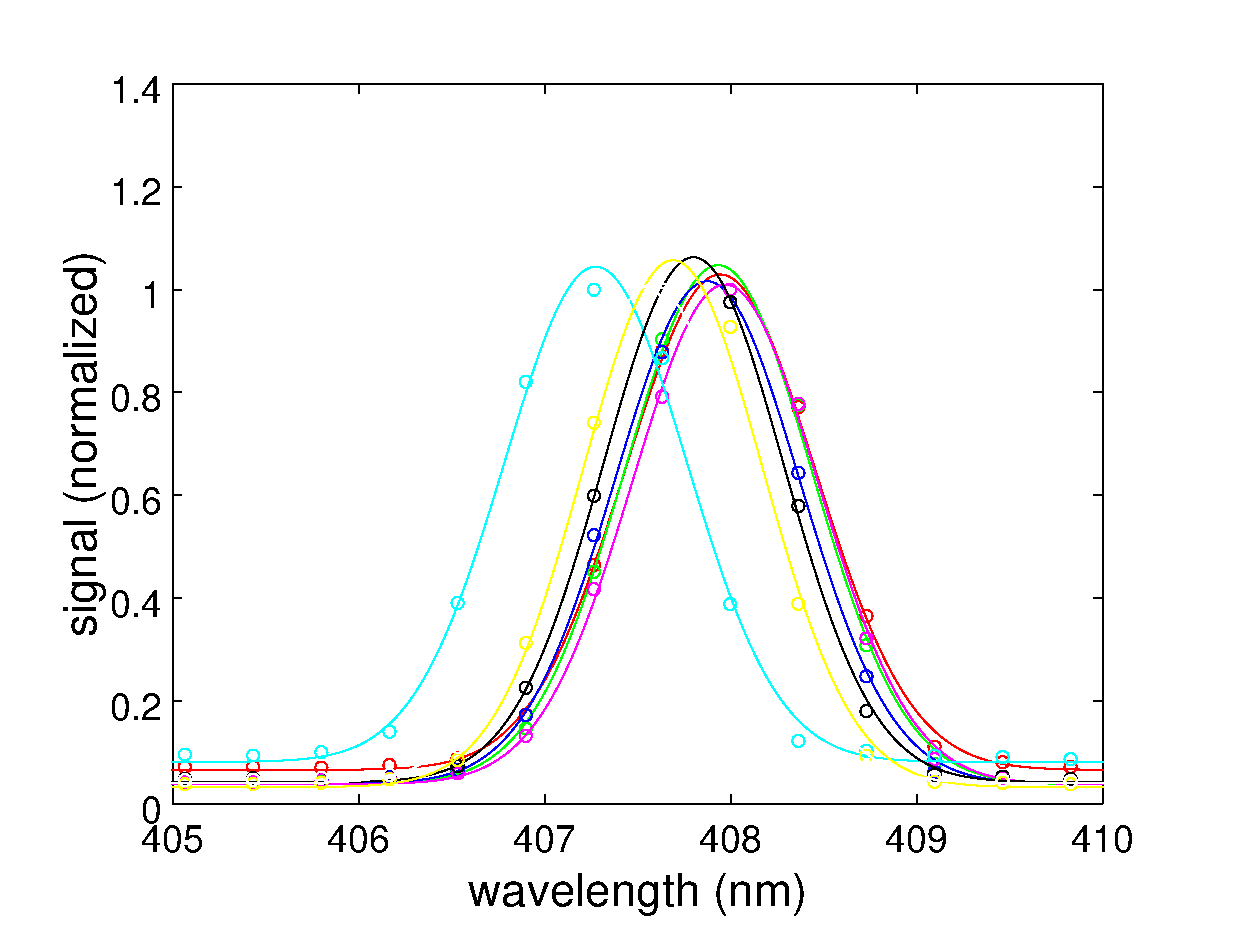
\includegraphics[width=0.95\textwidth]{wavelength_selected} 
\caption[Wavelength selected diodes]{\label{wavelengthselected} Representative data of the free-running (i.e. no grating feedback or extended cavity) wavelength of several wavelength selected lasers taken at 120 mA.} %temperature? %the ones we picked or someone else did? 
\end{figure}
\begin{figure}
\centering
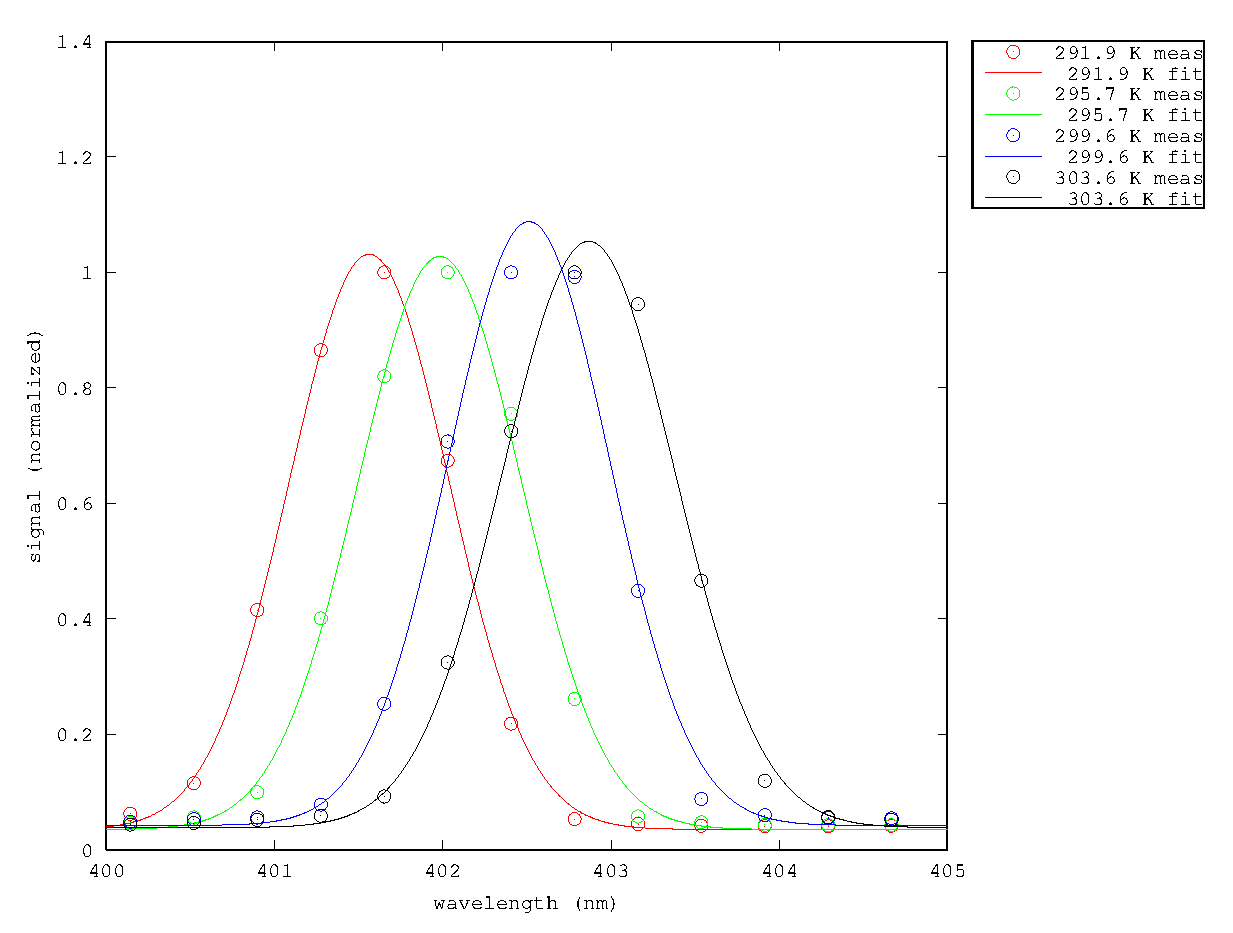
\includegraphics[width=0.95\textwidth]{temperatureFit} 
\caption[Wavelength of master laser at different temperatures]{\label{Temperaturespectra} Representative data of the free-running wavelength of our master laser as a function of temperature.}
\end{figure}

\subsection{Placement of the Grating}

%Some theory here might be worth reviewing. In addition, I did that really great mathematica notebook where I calculated all that stuff. 

%Installation of a diffraction grating allows us to selectively couple light of particular wavelengths back into 

Lasers work by amplifying light resonant with a particular mode of the laser cavity via stimulated emission. Ideally, we would like to favor a mode within the diode laser corresponding to our desired wavelength. In order to accomplish this, we add yet another resonant cavity outside our laser that can couple light back into the laser. 

This cavity is formed by a diffraction grating on one side and the entrance of the laser on the other side. This configuration is called an Extended Cavity Diode Laser (ECDL). The grating we selected was a Thorlabs model number GH13-36U, which has 3600 lines/mm. A picture of the grating can be seen in Figure\,\ref{diffractionGratingPhoto}. 

The diffraction grating is angled so that the first order diffraction peak at 407.771 nm light is directed back into the laser. The condition for this to be the case is 

\begin{equation} \label{gratingEQn}
n \lambda = 2 d \sin (\theta),
\end{equation}
where $n$ is the order of the diffraction peak (in our case, $n=1$), $d$ is the spacing between slits (in our case $d=1$ mm$/3600 = 278 $ nm) and $\theta$ is the angle of incidence to the grating. We can therefore calculate that the $\theta$ should be approximately
\href{http://www.wolframalpha.com/input/?i=arcsin%28+407.771+nm+%2F%282*%281+mm%2F3600%29%29%29+in+degrees}{$47.2^\circ$}.

 I machined a custom grating holder out of Aluminum, which can be seen in Figure\,\ref{master_laser_photo}. The aluminum holder was mounted in a Thorlabs KC1-PZ piezoelectric mount, which allows us the necessary fine control of the grating's location and angle over a narrow range of angles.  The grating was mounted approximately 4 cm from the aperture of collimating lens.
% The grating is mounted at such an angle that it selectively couples light with a wavelength near 408 nm back into the laser cavity. The resonant space between the diffraction grating and the collimating lens is what the phrase ``extended cavity'' refers to. The additional boundary conditions imposed on the resonant modes of the laser by the external grating result in a narrowing of the laser's linewidth. 
I had to ensure that the diffraction grating is installed such that both the angle and the cavity length match our desired wavelength. In order to get the grating aligned initially, I turned on the current to the laser until the laser was just below the threshold where it would begin to lase. We then aligned the grating using the threaded actuators on the piezoelectric mount until we saw the output power of the laser increase. When this happens, it indicates that we are successfully coupling light to the laser cavity. The output power of the laser can be monitored by eye or by instrument and it is fairly easy to get a feel for what it should look like when the grating first couples to a laser operating just below threshold. After light is coupling, I often again turn the current even lower and try to get the laser to lase at an even lower current. This process can be repeated several times in order to maximize the coupling of the light from the grating back to the laser.

After this, I used a Bristol 521 wavelength meter to measure the wavelength. The Bristol 521 is a calibrated instrument that relies on an optical Michelson-Morley interferometer to make measurements. (We used the grating spectrometer method instead of the Bristol 521 for the free-running lasers because the free-running lasers' linewidths was too large to be successfully measured on the wavelength meter.) Using the wavelength information from the wavelength meter, the laser is tuned iteratively by adjusting the grating using the threaded/manual actuators. For each adjustment, I then find new sets of currents at which the laser will operate stably. 

%did I ever tune it to the right wavelength using the Bristol wave meter? 
\subsection{Ensuring Ability to Fine Tune}

The piezoelectric actuators on the grating mount can also be moved electrically. It is important that we find a way to move the piezeoelectric actuators in concert in such a way that we maximize the range over which we can scan the laser frequency without the laser mode hopping. When the $^{87}$Sr$^+$ ion interferometer is operational, we might need this for several reasons: First, it may be the case that we decide to lock the laser to an external reference like a vapor cell or a cavity. In this case, the laser frequency will need to be adjusted based on an error signal that we derive from our stable reference. In the current setup, we do not lock the laser to any external reference (we probably do not need to since we plan to operate the lasers fairly far from the resonance and the system has been show to be relatively insensitive to the overall frequency). However, we never know if we might decide we want to on some later date. Second, the ability to modulate the laser with a single knob is very handy. In fact, this is what we did to verify that the slave laser frequencies were properly tracking with the master laser frequency (see Fig.\,\ref{fig:slaveMaster}). Experimenters running the ion interferometer experiment will likely appreciate a simple way to tune the laser manually that does not involve rather having to adjust several pieces separately. 

%The grating setup is also crucial in order to allow the master laser to be tuned. Therefore, the piezoelectric actuators can be connected to control circuitry that can be used to tune the laser based on a signal derived from transmission through a Strontium vapor cell. 

The control circuitry will be similar to the PID controllers desribed in Ref.\,\cite{cjeDiss} that are used elsewhere in the lab (see Fig.\,\ref{circuit}). These PID controllers consist of a simple PID controller combined with a ``scan balancer.'' The PID controller segment of the circuit could be used to generate a feedback signal based on an error signal. We could generate suitable error signals by measuring absorption through a vapor cell or by looking at transmission through a cavity. The scan balancer takes the feedback signal and allows us to use it to generate three signals with independently-controllable gains: one signal can be used to modulate the current coming from the laser current driver. The other two signals can be amplified and sent to the piezoelectric actuators.  The circuit also features a DC offset that can be digitally controlled and added directly to the feedback signal. Thus, if the scan balancer is configured with suitable gains, the experimenter can make fine adjustments to the tuning of the master laser using a digital control knob.

\begin{figure}
\centerline{
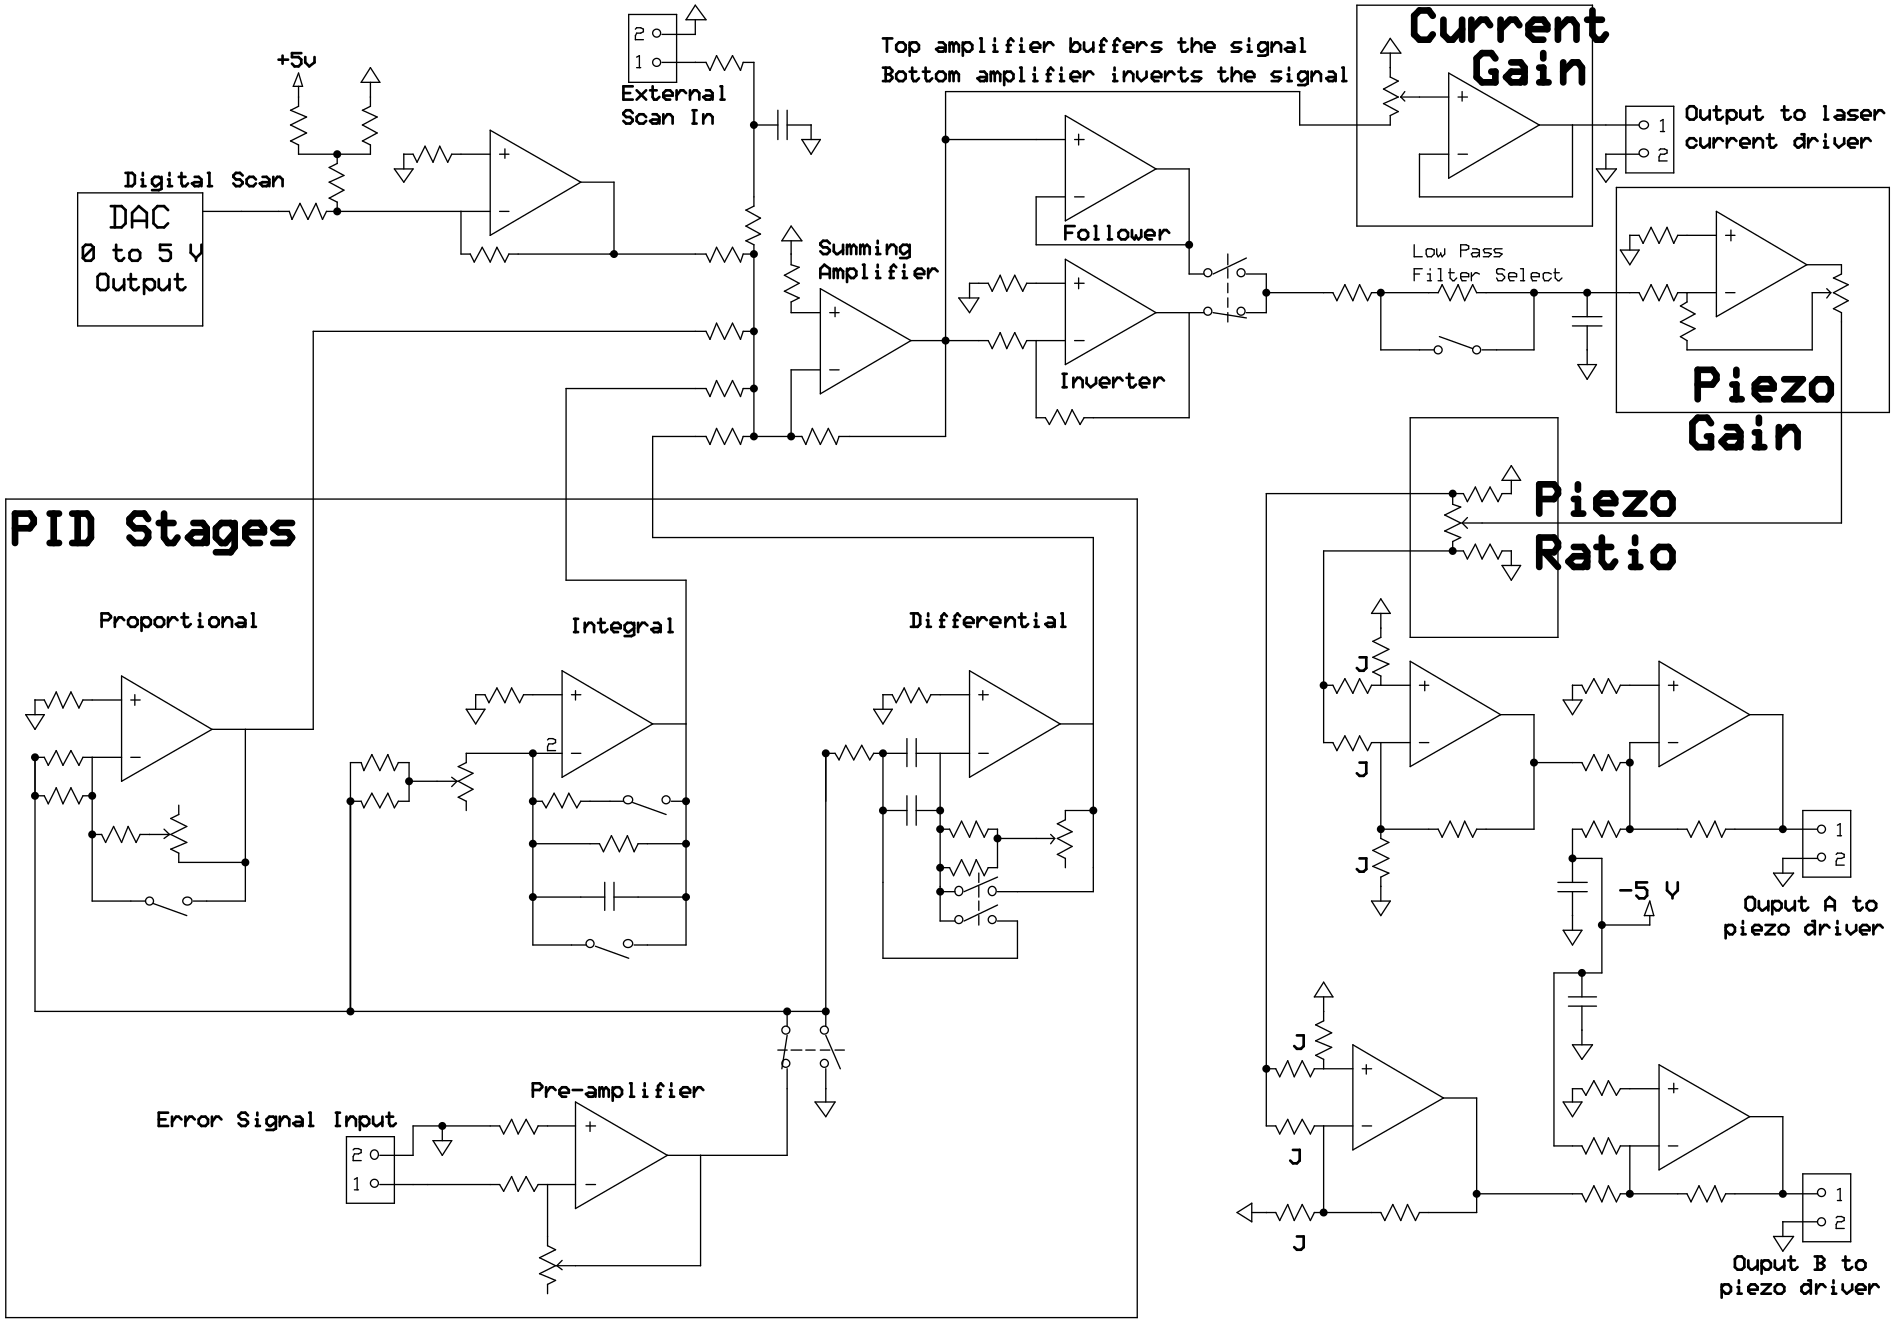
\includegraphics[width=0.95\textwidth]{PID from cje diss.png}}
\caption[Schematic of PID circuit]{\label{circuit} Schematic of the PID circuit developed by others in the lab that we use on the master laser. The PID stages are depicted at the bottom left of the diagram and these will be used only if we lock the laser system to an external reference. At the top left of the diagram is a DAC that allows us to set a digital offset. The signal from this DAC is added directly to the feedback signal that comes out of the PID stages. Even if we do not lock the laser to a vapor cell, we can a do use the DC offset signal. }
\end{figure}

%However, even if we do not lock the laser to some external reference, the PID controller described in Ref.\,\cite{cjeDiss} also contains a series of amplifiers that take the feedback signal us to easily modulate the current of the laser along with the This feedback signal can then be used to control the voltage on the piezoelectric actuators along with the current to the laser. The PID controller's output stage allows the user to select various gains that control the movement of each of the piezoelectric actuators. However, even if we do not use the PID control features, 
%did I ever tune this up? 

%todo: figure out whether we need to lock it to a cell. 
However, in order for this to work, we must properly set the gains in the scan balancer. here is some insight to be gained by modeling the ideal relative motion of the piezoelectric actuators that will ensure that the grating moves in such a way that the resonance of the cavity it creates changes as smoothly as possible over as wide a range of wavelengths as possible. 


%Our goal is to ensure that the grating moves in such a way that the resonance of the cavity it creates changes as smoothly as possible over as wide a range of wavelengths as possible. 

The change in the wavelength reflected from the grating as a function of $\theta$ can be found by taking the derivative of Eq.\,\ref{gratingEQn} with $n=1$:

\begin{equation}
    \frac{d\lambda}{d \theta}= \frac{2d}{\lambda} \cos(\theta)
\end{equation}.

However, as we move the grating, we also want to make sure that the cavity length ($L$) changes in such a way that $L/\lambda$ remains constant. 

\begin{equation}
    \frac{d \lambda}{d L}= \textnormal{constant} 
\end{equation}

We note that $L$ and $\theta$ are both functions of the piezo actuators. The geometry is straightforward, but involves a lot of terms. We model this in a well-commented Mathematica Notebook included in Appendix\,\ref{GratingRatioAppendix}. The ratio that we find to be about right is 0.478755. In practice, we would fine tune this ratio by scanning the piezos and iteratively making adjustments to maximize the size of the range over which the laser operates single mode. However, the calculation is nice to have since it gives a good starting point and some geometries result in surprising ratios (for example, one of the lasers discussed in Ref.\,\cite{cjeDiss} required that the piezos scan in opposite directions, which required a change to the scan balancer circuitry).


\subsection{Calculation of Maximum Safe Intensity}

The specifications in the datasheet for the laser diode are valid only when the diode is free running. However, using the laser in an ECDL configuration requires coupling power back into the laser diode. In order to ensure that we did not damage our laser, we performed a brief calculation. We assumed that the maximum current for which the diode is rated corresponds to the maximum amount of power that can be emerging through the front facet of the laser without damage. We put the maximum recommended current of 250 mA through the laser and measured the output. Then we measured the efficiency of the grating. From this, we were able to model the external cavity and deduce how much power would be coming out of the the cavity when the power coming out the front face of the laser was near its maximum allowable value. We then measured the output of the cavity for various currents. We estimated that it is safe to run the laser at currents up to $\sim$105 mA. 
%todo: look this up more
%calculation is in part II page 20 

%TODO: look at the peaks of the laser cavity that you did before when Dallin said ``You better make good notes and put that in your thesis''
 
\section{Operation}

The master laser successfully runs single mode. It has been tuned to the correct 407.771 nm wavelength with the Bristol Wavemeter while operating single mode with grating feedback with a temperature of 26.798$^\circ$C and a current of 65.9 A. It produces 19 mW of power. 

%should I discuss how we tuned it to the Bristol Wavemeter? 



